\documentclass[final]{beamer}

% ====================
% Packages
% ====================

\usepackage[T1]{fontenc}
 \usepackage[utf8]{luainputenc}
\usepackage{lmodern}
\usepackage[size=custom, width=120,height=90, scale=1.32]{beamerposter}
\usetheme{gemini}
\usecolortheme{cam}
\usepackage{graphicx}
\usepackage{booktabs}
\usepackage{tikz}
\usepackage{pgfplots}
\pgfplotsset{compat=1.14}
\usepackage{anyfontsize}
\usepackage{fontawesome5}
\usepackage{algorithm}
\usepackage{algpseudocode}
\usepackage[backend=biber,style=ieee]{biblatex}

% \directlua{ require("drawboxes")}
% \AtBeginShipout {\directlua{drawboxes.visual_debug()}}

\usetikzlibrary{shapes,arrows,positioning,calc}
\tikzset{block/.style={
        font=\sffamily,
        draw=black,
        thin,
        fill=pink!50,
        rectangle split,
        rectangle split horizontal,
        rectangle split parts=#1,
        outer sep=0pt},
        %
        gblock/.style={
            block,
            rectangle split parts=#1,
            fill=green!30},
        yblock/.style={
            block,
            rectangle split parts=#1,
            fill=yellow!30}
        }

\addbibresource{references.bib}

\graphicspath{{../figures/}}

% ====================
% Lengths
% ====================

% If you have N columns, choose \sepwidth and \colwidth such that
% (N+1)*\sepwidth + N*\colwidth = \paperwidth
\newlength{\sepwidth}
\newlength{\colwidth}
\setlength{\sepwidth}{0.025\paperwidth}
\setlength{\colwidth}{0.3\paperwidth}

\setlength{\floatsep}{1pt plus 2.0pt minus 2.0pt}
\setlength{\intextsep}{1pt plus 2.0pt minus 2.0pt}
\newcommand{\squeezeup}{\vspace{-20.5mm}}

\newcommand{\separatorcolumn}{\begin{column}{\sepwidth}\end{column}}
\renewcommand*{\bibfont}{\footnotesize}

% ====================
% Title
% ====================

\title{\Large Practical Analysis of Hybrid Sorting Algorithms}

\author{\large Joshua Arulsamy, Dr. Lars Kotthoff\\
	\normalsize \texttt{jarulsam@uwyo.edu}, \texttt{larsko@uwyo.edu}
}

\institute{Department of Electrical Engineering and Computer Science, University of Wyoming}

% ====================
% Footer (optional)
% ====================

\footercontent{}
% (can be left out to remove footer)

% ====================
% Logo (optional)
% ====================

% use this to include logos on the left and/or right side of the header:
% Left: institution
 \logoleft{
\includegraphics[height=2.9cm]{logos/New_UWSignature_1_line_White_Web.png}}
% Right: funding agencies and other affilations
% \logoright{
\includegraphics[height=2.5cm]{logos/WRSP/abbreviated/UWabbreviated_V_WRSP_white.png}}
% ====================
% Body
% ====================

\begin{document}

\addtobeamertemplate{block begin}{\vskip -6mm}{}
\addtobeamertemplate{block end}{}{\vskip -6mm}

\begin{frame}[t]
	\begin{columns}[t]
		\separatorcolumn

		\begin{column}{\colwidth}

			\begin{block}{Introduction}
				\begin{itemize}
					\item The procedure of reordering data according to some comparator is
					      called sorting. Sorting can be found in nearly every computer
					      system today.
					\item The near omnipresent need for performant sorting implementations
					      has resulted in most major programming languages including a
					      type-generic sorting function within their standard libraries.
					\item This research analyzes a wide variety of sorting algorithm
					      implementations across varying system architectures to determine
					      optimal parameter configurations for hybrid sorting algorithms.
					\item This research also proposes a new performant standard sorting
					      implementation for GNU's C standard library leveraging,
					      Mergesort, insertion sort, and sorting networks.
				\end{itemize}
			\end{block}

			\begin{block}{Background}
				\begin{itemize}
					\item Substantial effort has been spent on the analysis of sorting
					      algorithms. Typically, two major characteristics are considered
					      when studying sorting algorithms; space and time
					      complexity\parencite{Bentley1993EngineeringAS}.
					\item Existing analysis of popular sorting algorithms, such as
					      Quicksort and Mergesort, place substantial emphasis on their
					      excellent asymptotic complexity in the average
					      case\parencite{glibc}.
					\item Asymptotic complexity alone does not describe the practical
					      performance of these algorithms. While Mergesort may have a
					      better asymptotic time complexity in the worst case than
					      insertion sort, for small inputs, insertion sort typically
					      outperforms Mergesort by avoiding the overhead of recursive
					      calls.
				\end{itemize}
			\end{block}

			\begin{block}{Proposed Algorithm}
				\begin{itemize}
					\item The proposed algorithm is a highly-optimized version of
					      Mergesort leveraging both insertion sort and a network sorting
					      algorithm.
					\item During recursive calls of conventional Mergesort, if the
					      subarray's length is less than a threshold value, insertion sort
					      is used instead.
					\item In instances where a subarray contains less than 5 elements, a
					      comparison-optimal network sorting algorithm is used instead.
				\end{itemize}
				\vspace{-8mm}

				\def\lvld{3.0}                  % Choose level distance
				\pgfmathsetmacro\shft{-4*\lvld} % Calculate the yshift for the green tree
				\begin{figure}[h]

					\begin{minipage}{0.45\textwidth}
						\centering
						\begin{tikzpicture}[level distance=\lvld cm,
								level 1/.style={sibling distance=6cm},
								level 2/.style={sibling distance=3cm},
								edgedown/.style={edge from parent/.style={draw=red,thick,-latex}},
								edgeup/.style={edge from parent/.style={draw=green!50!black,thick,latex-}}
							]

							% GREEN TREE (drawn first to let the middle line filled in pink)
							\node[gblock=4,yshift=\shft cm] (A') {1 \nodepart{two} 2 \nodepart{three} 3 \nodepart{four} 4}
							[grow=up,edgeup]
							child {node[gblock=2] (B2') {1 \nodepart{two} 4}
									child {node[yblock=1] (D6') {1}}
									child {node[yblock=1] (D5') {4}}
								}
							child {node[gblock=2] (B1') {2 \nodepart{two} 3}
									child {node[yblock=1] (D2') {2}}
									child {node[yblock=1] (D1') {3}}
								};

							% PINK TREE
							\node[block=4] (A) {3 \nodepart{two} 2 \nodepart{three} 4 \nodepart{four} 1} [grow=down,edgedown]
							child {node[block=2] (B1) {3 \nodepart{two} 2 \nodepart{three}}
									child {node[yblock=1] (D1) {3}}
									child {node[yblock=1] (D2) {2}}
								}
							child {node[block=2] (B2) {4 \nodepart{two} 1}
									child {node[yblock=1] (D5) {4}}
									child {node[yblock=1] (D6) {1}}
								};
						\end{tikzpicture}
						\centering
						\label{fig:mergesort}
						\caption{Mergesort, 8 comparisons}
					\end{minipage}\hfill
					\begin{minipage}{0.50\textwidth}
						\centering
						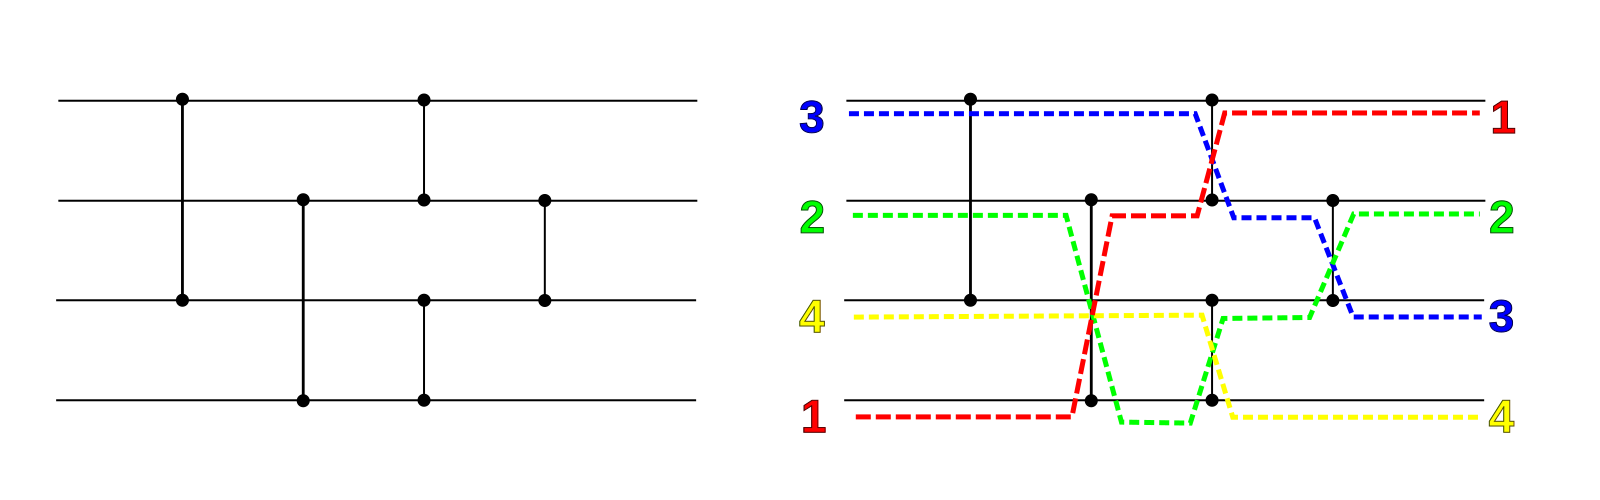
\includegraphics[trim={21cm 0 0 0},clip,width=\textwidth]{SimpleSortingNetworkFullOperation}
						\vspace{10mm}
						\caption{Sorting network, 5 comparisons}
						\label{fig:sortingnetwork}
					\end{minipage}\hfill
				\end{figure}

				\vspace{-8mm}
				\begin{itemize}
					\item Sorting networks deterministically sort small quantities of
								items extremely efficiently. In this example, a sorting network
								(Fig. \ref{fig:sortingnetwork}) avoids three unnecessary
								comparisons made by Mergesort (Fig. \ref{fig:mergesort}).
				\end{itemize}
			\end{block}

		\end{column}

		\separatorcolumn

		\begin{column}{\colwidth}

			\begin{block}{Experimental Setup}

				\begin{itemize}
					\item A small subset of algorithms is chosen for evaluation
					\item Algorithms utilized within standard library implementations are
					      of particular interest, since they are typically highly
					      performant in the general case.
					\item Other complementary algorithms which perform exceptionally well
					      in specific scenarios are also evaluated.
					\item General purpose sorting function are taken from various standard
					      libraries, such as GNU's libc\parencite{glibc} and musl
					      libc\parencite{musl_libc}.
				\end{itemize}
				\begin{enumerate}
					\item \textbf{Each algorithm is timed while sorting the same data
						      using a variety of threshold values.} This is repeated 1,000
					      times. The mean is calculated for each algorithm. This is done
					      to minimize noise (time inaccuracy, other processes on the test
					      system, etc.) during data collection.
					\item \textbf{Each algorithm configuration is tested on a variety of
						      platforms}. To determine whether the algorithms perform well
					      across a variety of architectures, each test is repeated on
					      several different commonly used systems.
				\end{enumerate}
			\end{block}

			\begin{block}{Results}
				\begin{itemize}
					\item The proposed algorithm (Mergesort w/ Fast InsSort \& Network)
					      outperforms all other evaluated algorithms in most scenarios.
					      Most notably, entirely random data (Fig. \ref{fig:random}) sees
					      an upward of 15\% runtime reduction.
					\item Some platforms see little improvement with the additional
					      hybridization of networking sorting, while others see
					      significant performance gain (Fig. \ref{fig:randomvariance}).
					\item This indicates an area in need of further investigation.
				\end{itemize}

				\begin{figure}[h]
					\centering
					\makebox[\colwidth]{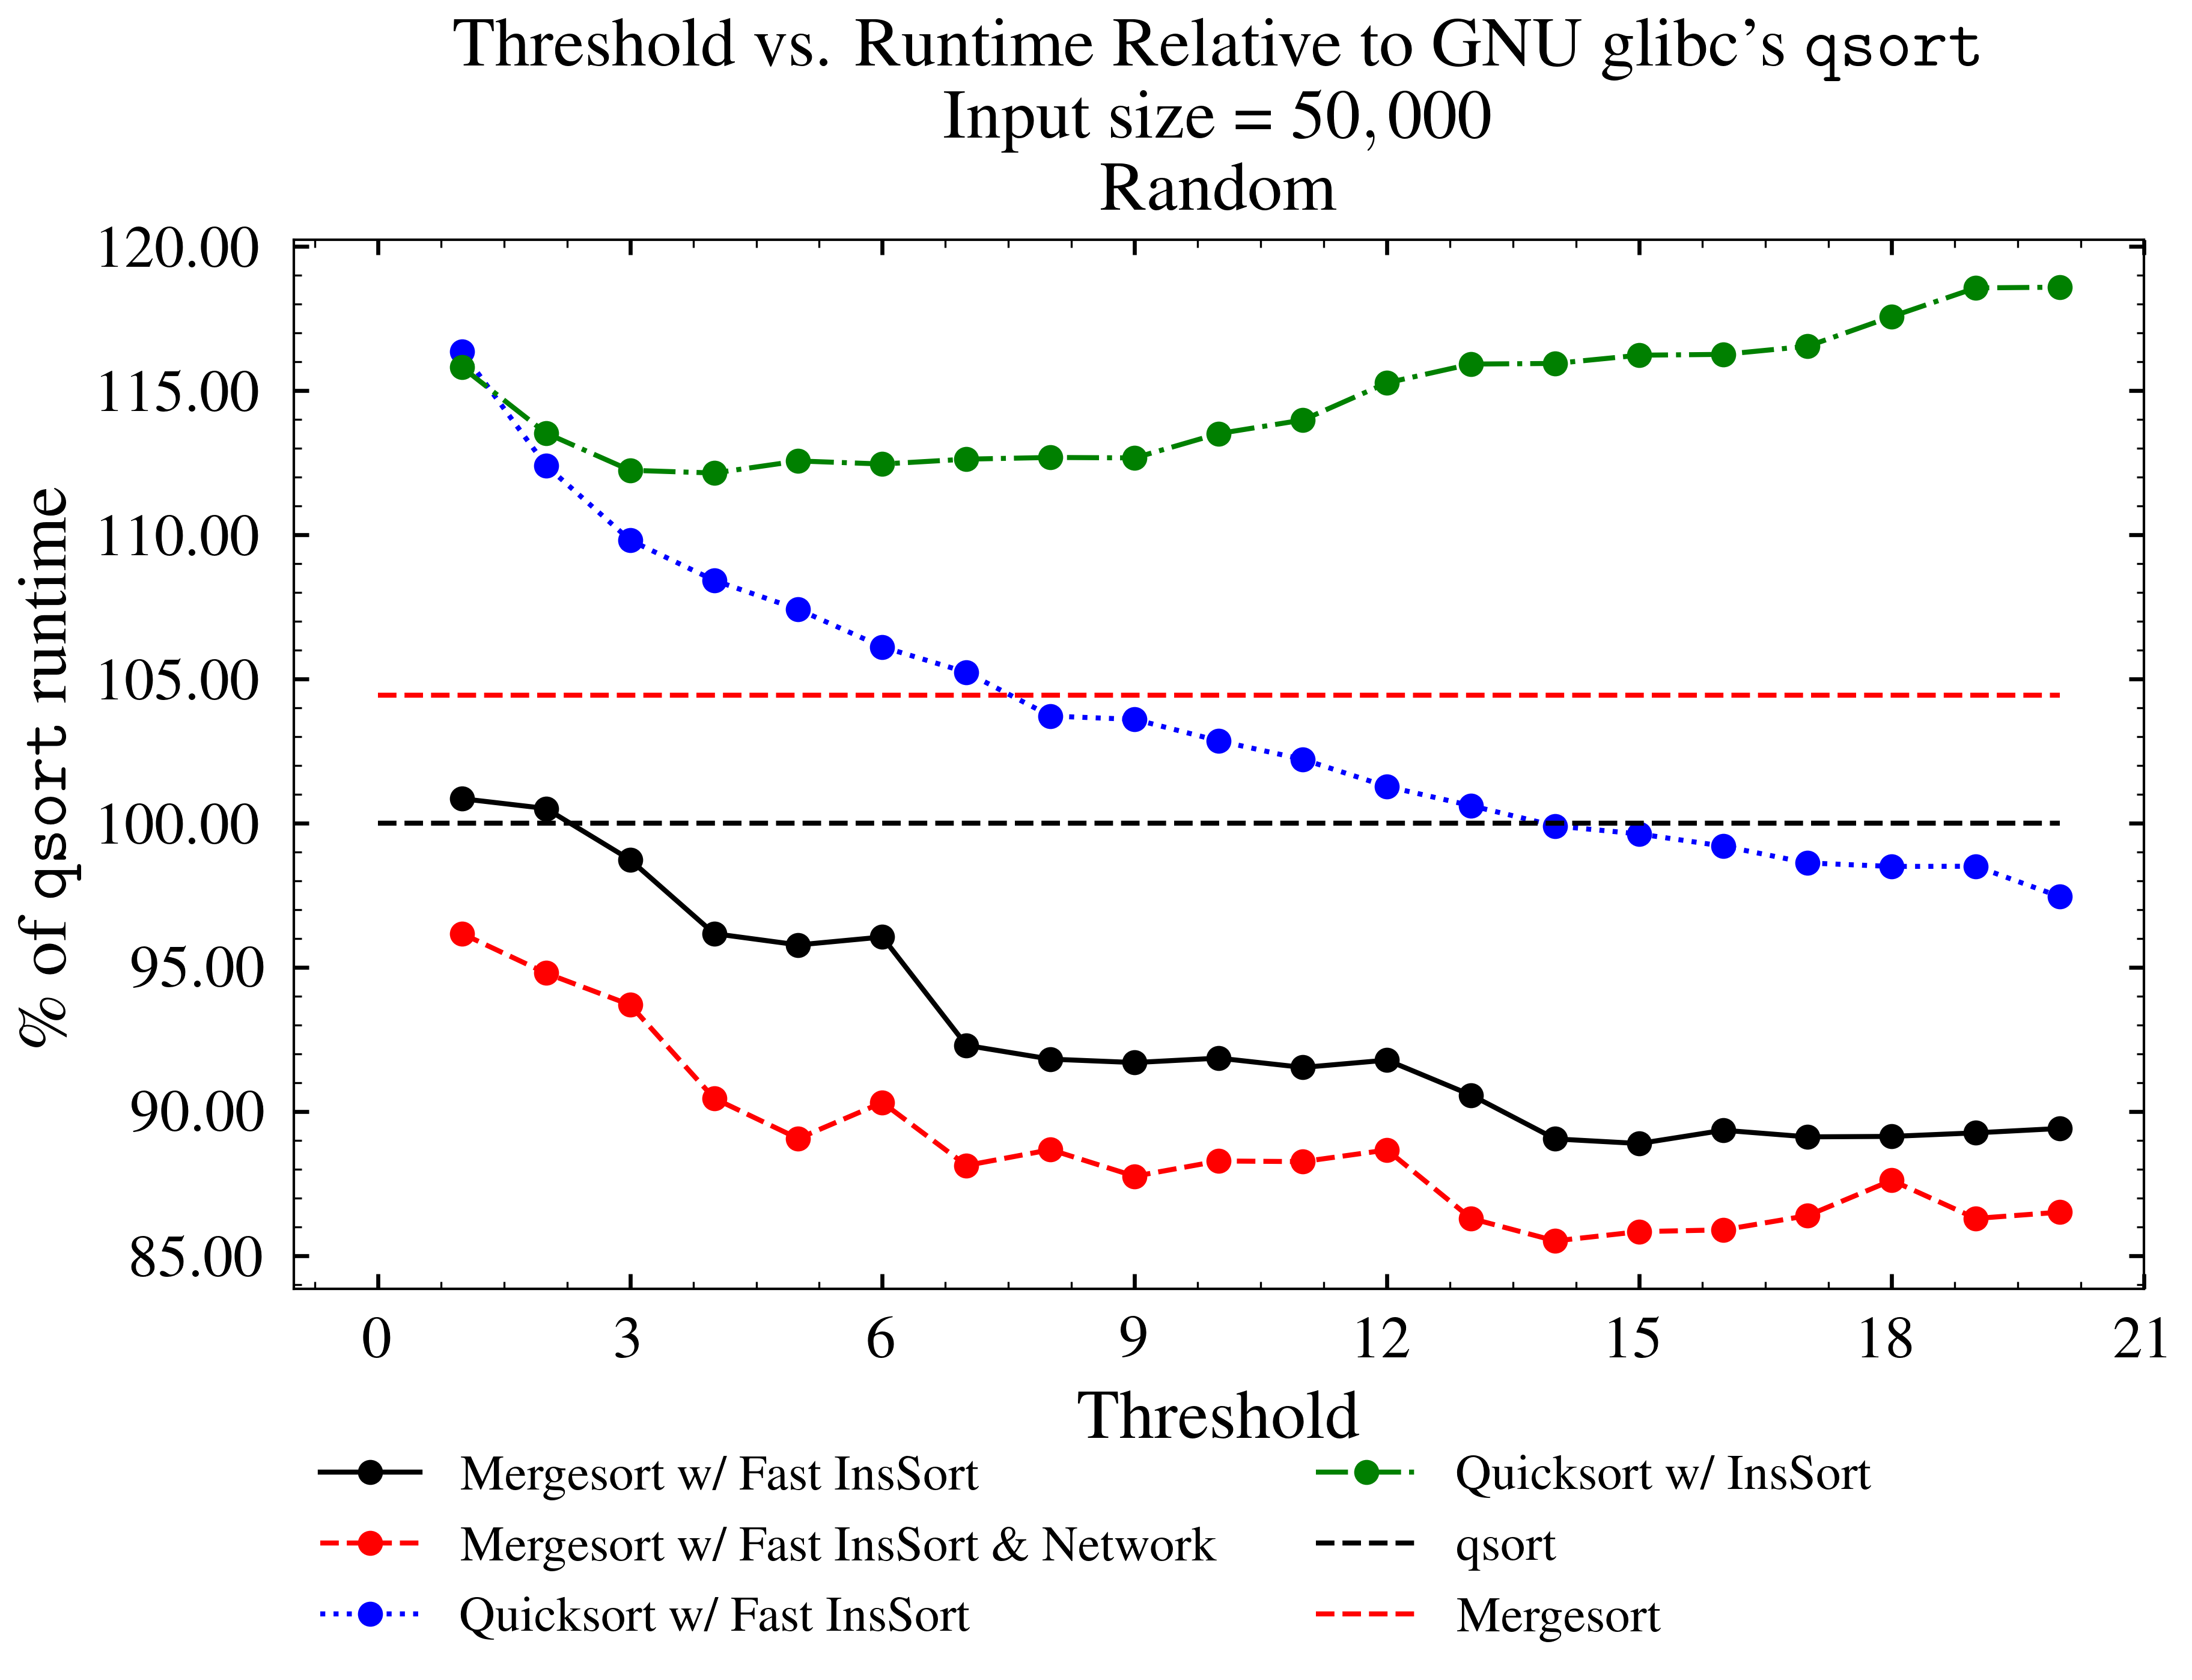
\includegraphics[width=\colwidth]{random}}
					\vspace*{-22mm}
					\caption{Runtime vs. Threshold on Random Input Data}
					\label{fig:random}
				\end{figure}
			\end{block}
		\end{column}

		\separatorcolumn

		\begin{column}{\colwidth}

			\vspace{11.5mm}
			\begin{block}{}
				\begin{figure}[h]
					\centering
					\makebox[\colwidth]{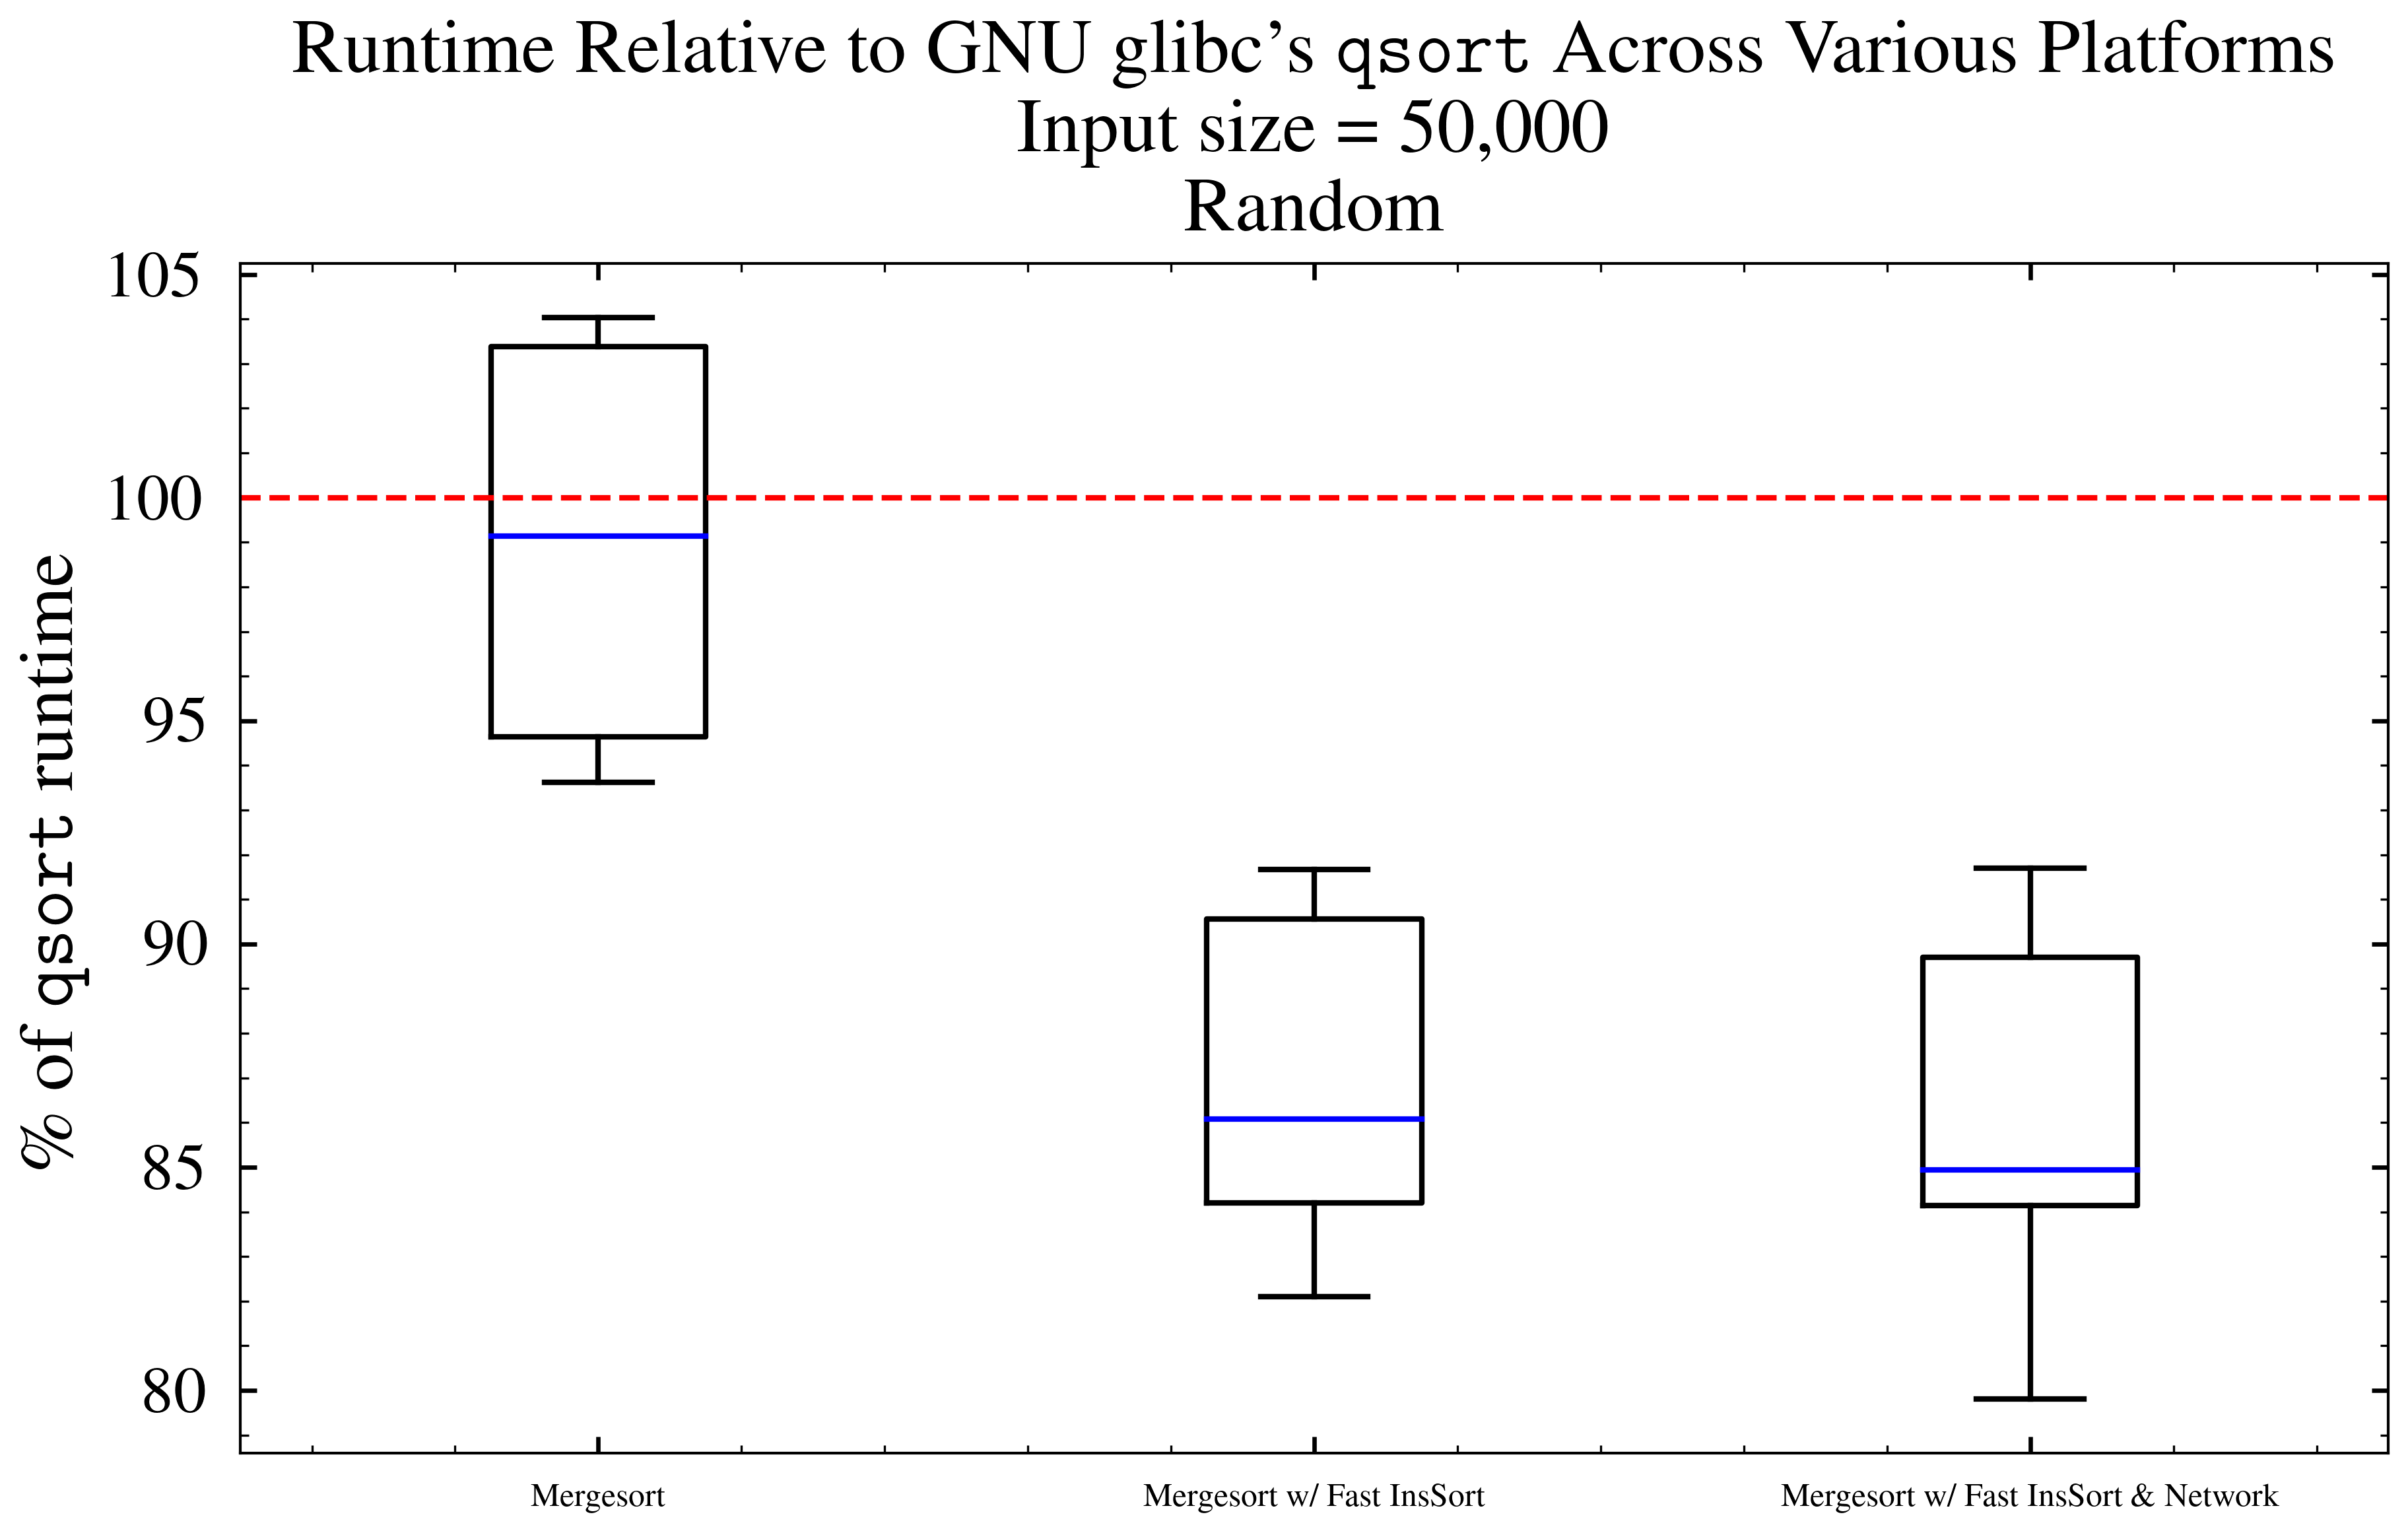
\includegraphics[width=\colwidth]{boxplots/4.gen}}
					\caption{Best Runtime By Method Across Various Platforms on Random Input Data}
					\label{fig:randomvariance}
				\end{figure}
			\end{block}

			\begin{block}{Conclusion}
				\begin{itemize}
					\item Clever usage of several specialized algorithms can offer better
					      general performance.
					\item Large scale testing utilizing super-computing resources from
					      ARCC can offer great insight of algorithm performance in a wide
					      variety of scenarios\parencite{ARCC}.
					\item Sorting, while considered a mostly solved problem, still has
					      areas in need of exploration.
					\item More specific testing utilizing profilers and other advanced
					      tools may lead to even faster implementations.
					\item All testing and implementation code is available online:
					      \href{https://github.com/uwyo-mallet/Hybrid-Sorting-Optimization}{https://github.com/uwyo-mallet/Hybrid-Sorting-Optimization}
				\end{itemize}
			\end{block}

			\begin{block}{Acknowledgments}
				This research would not have been possible without the guidance and
				gracious support by those listed below.
				\vspace{-5mm}
				\begin{itemize}
					\item Dr. Lars Kotthoff \& The MALLET Lab
					\item Wyoming Research Scholars Program
					\item The ARCC Support Team
				\end{itemize}
			\end{block}

			\vspace{10mm}
			\nocite{ARCC}
			\begin{block}{References}
				\printbibliography
			\end{block}
		\end{column}

		\separatorcolumn
	\end{columns}
\end{frame}

\end{document}
